\chapter{Attachments}

\section{Source codes}
\xxx{TODO: add a brief recap of the source codes}

\section{GitHub}
\label{sec:github}

The source codes are publicly available on GitHub at \url{https://github.com/cusbg/prankweb}.

\section{Abbreviations}
\label{sec:abbreviations}

\xxx{TODO: maybe add abbreviations to the end?}

\section{Pocket detail designs}
\label{sec:pocket_detail_designs}

This section contains all pocket detail designs that were considered for displaying more information about a pocket. In the end, the \cref{fig:dialog-4} was chosen. For more information refer to \cref{sec:plugins}.

\begin{figure}[htb]
    \centering
    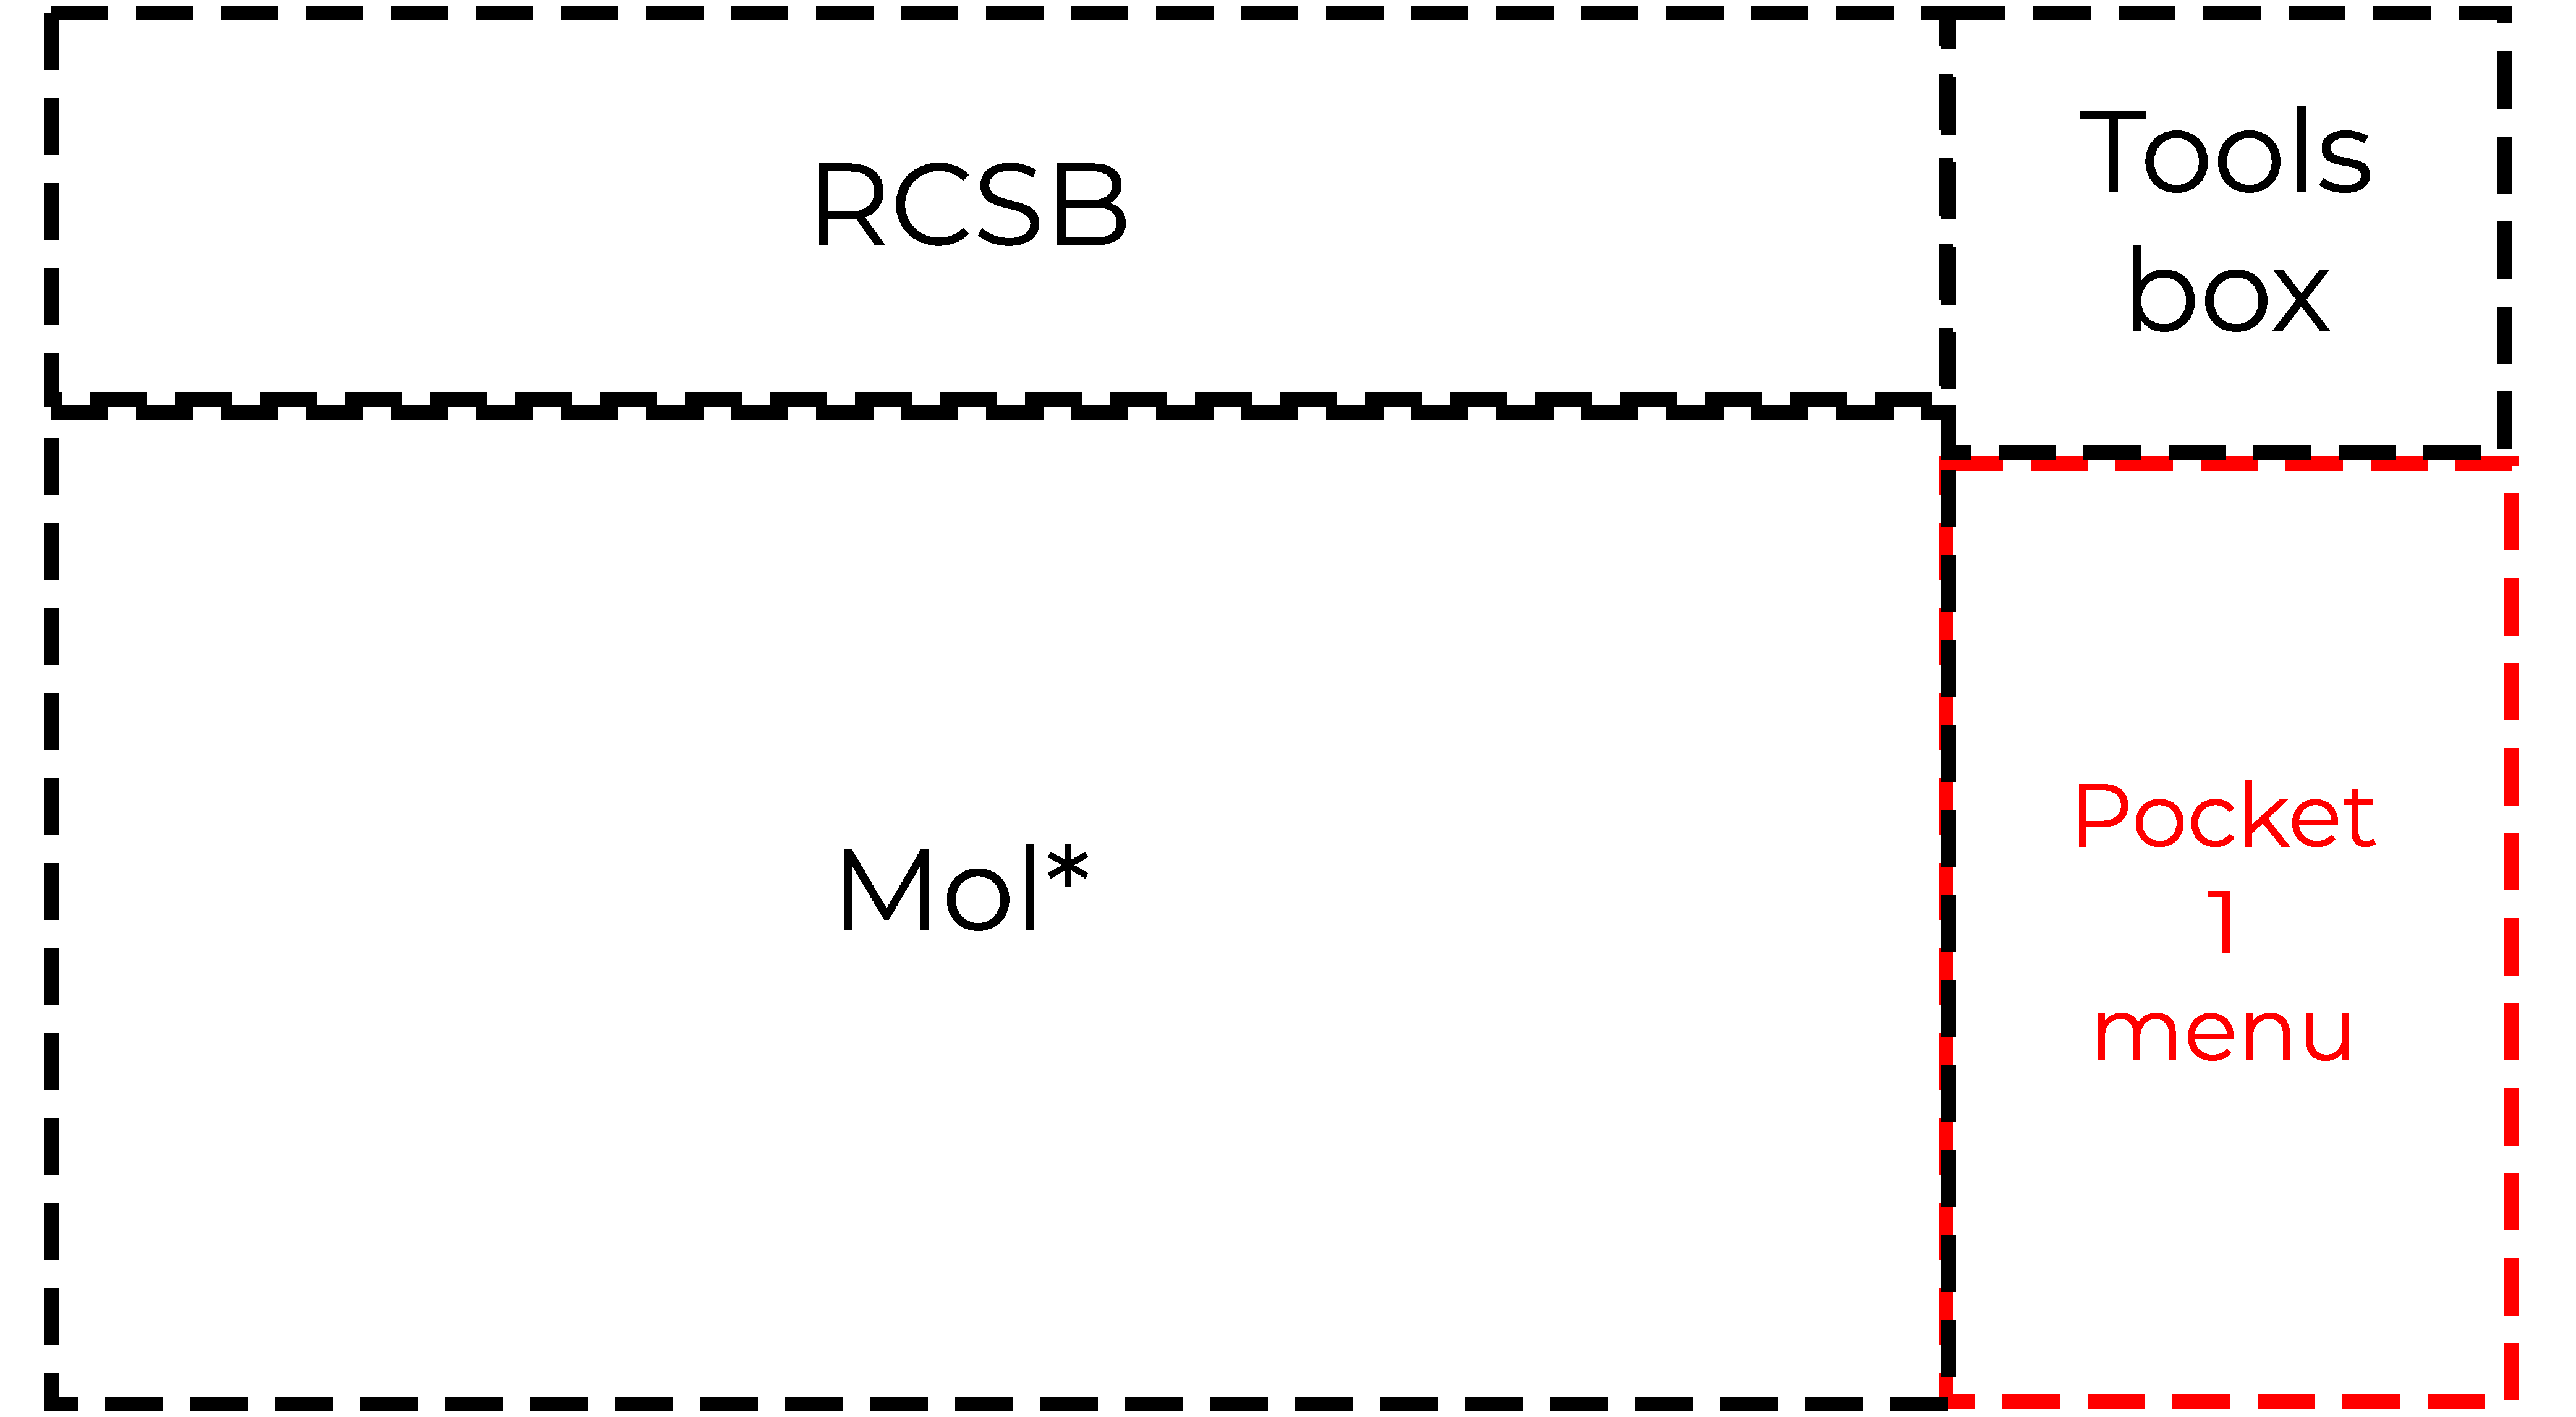
\includegraphics[width=\linewidth]{img/dialog_1-svg.pdf}
    \caption{The first option for displaying detailed pocket information. The tools box stays on the top, details of the chosen pocket are displayed in an extended box below. Other pockets are hidden.}
    \label{fig:dialog-1}
\end{figure}

\begin{figure}[htb]
	\centering
	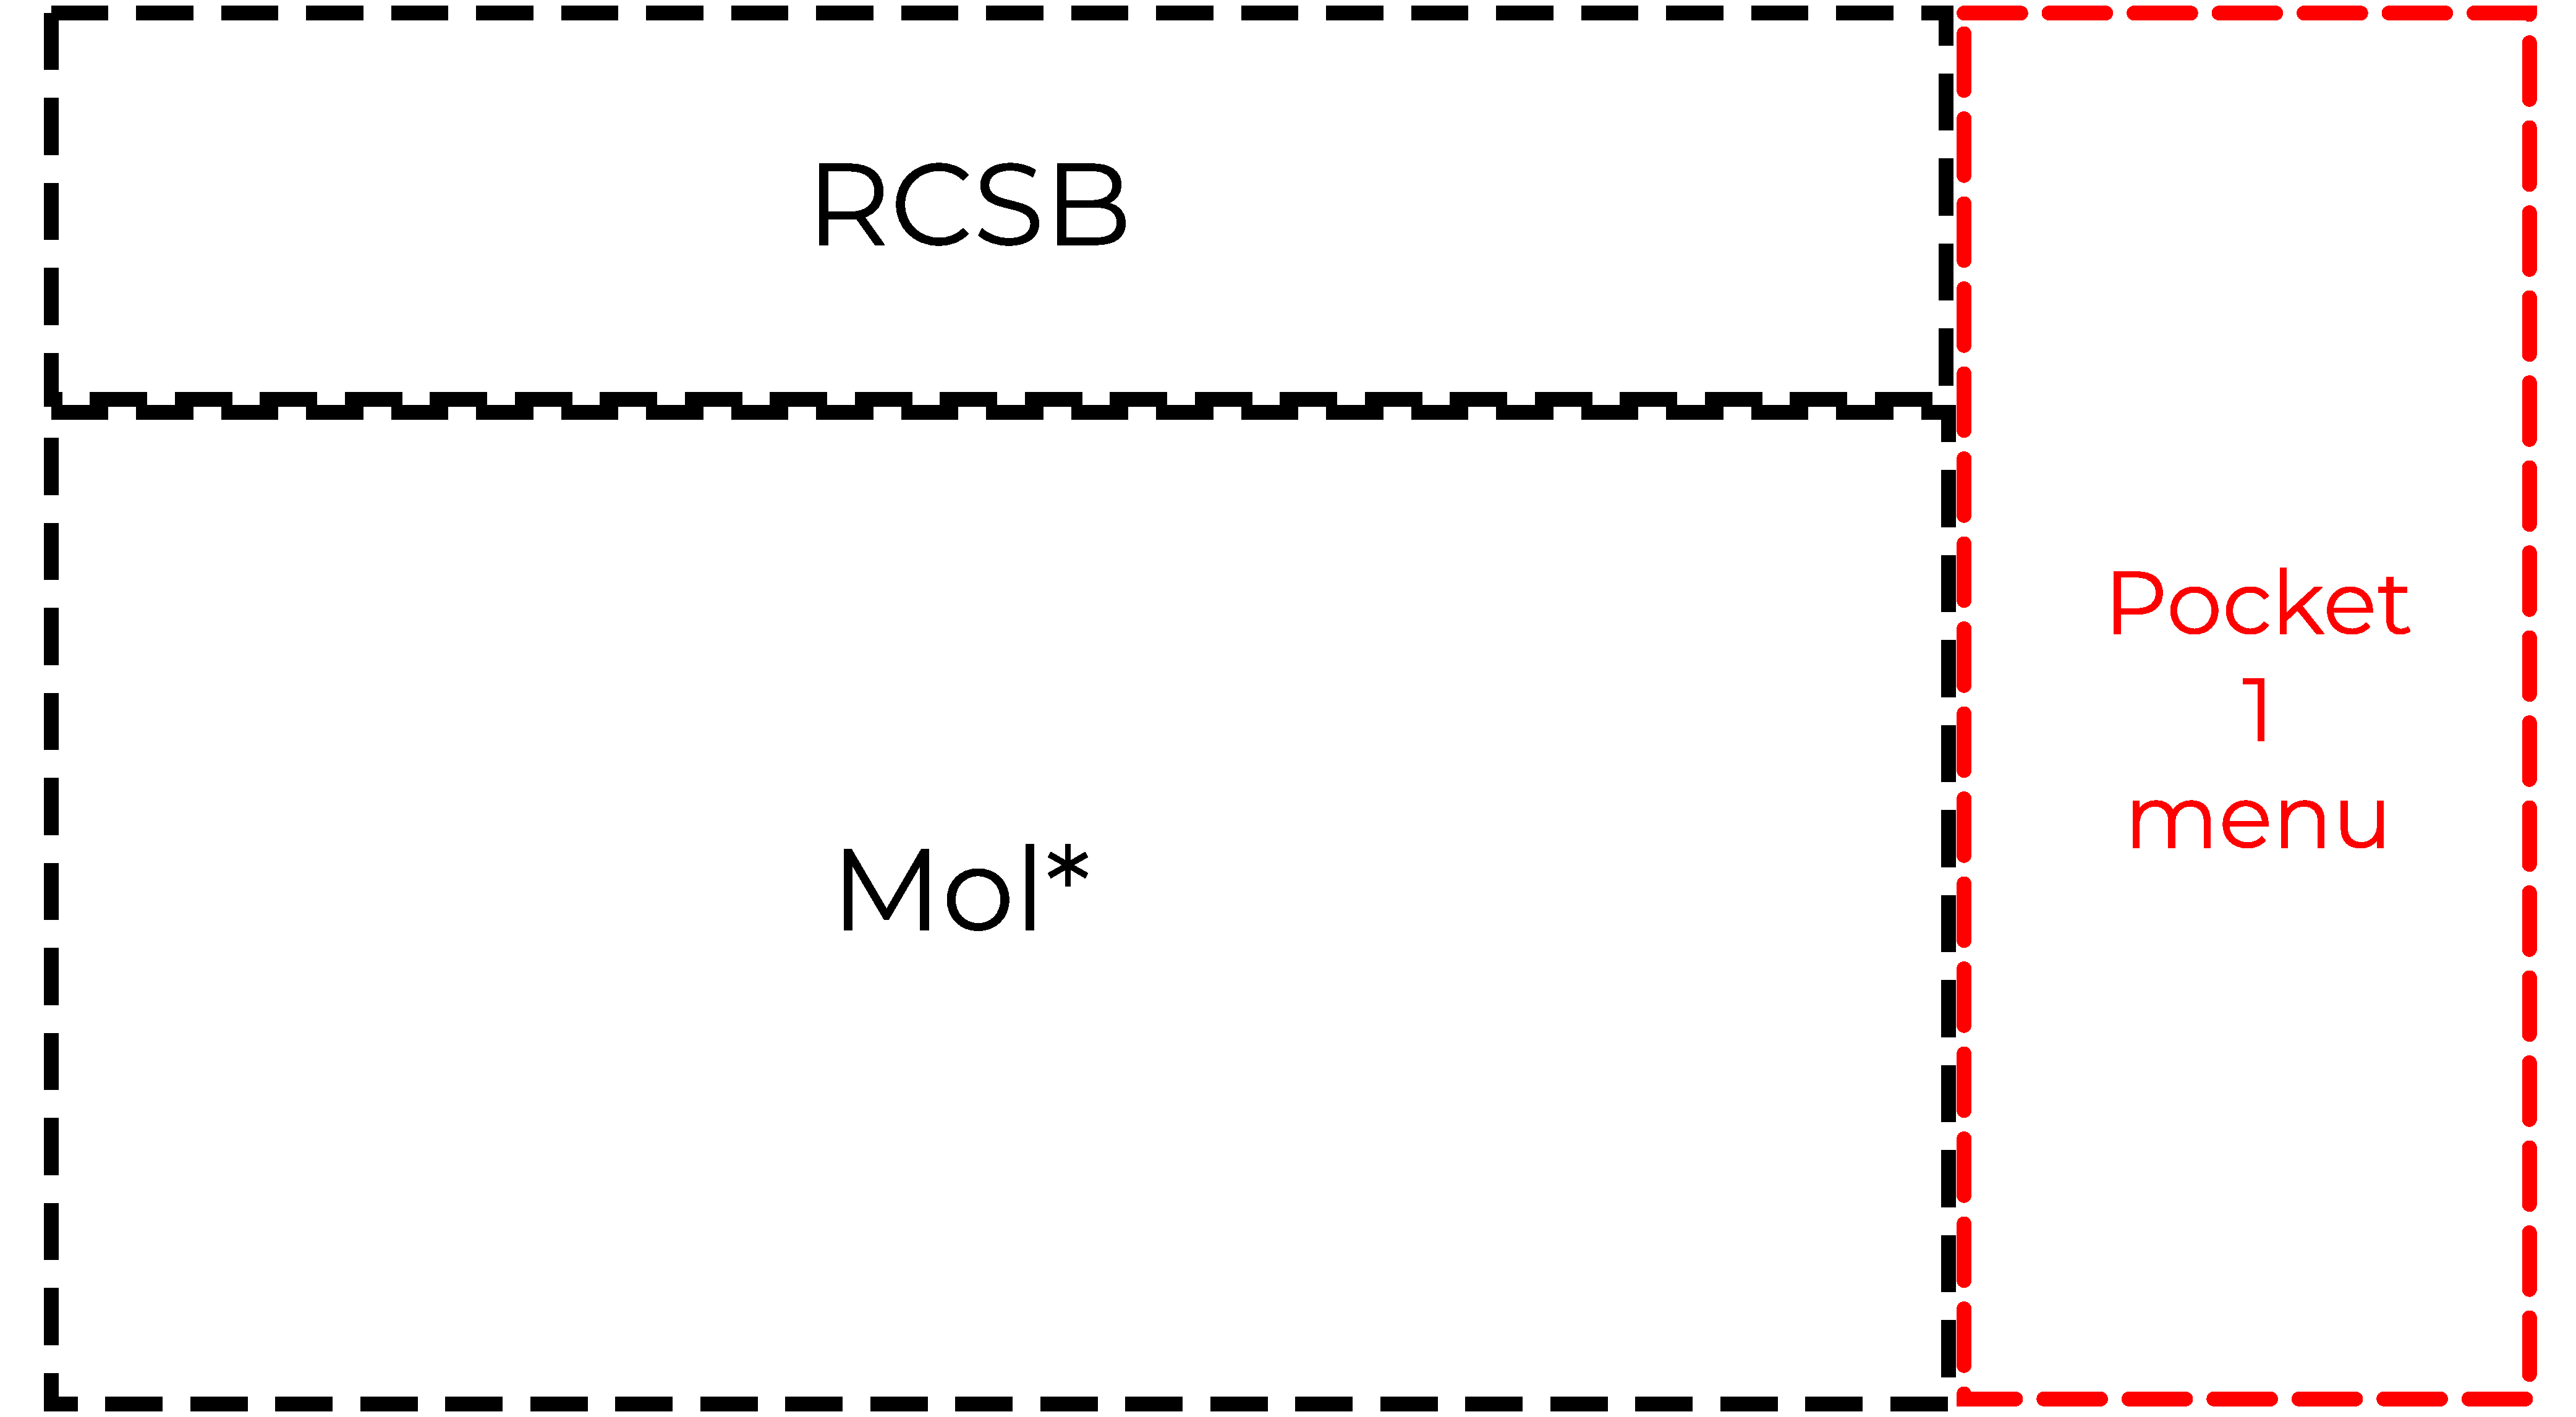
\includegraphics[width=\linewidth]{img/dialog_2-svg.pdf}
	\caption{The second option for displaying detailed pocket information. The tools box is hidden as well as other pockets, details of the chosen pocket cover the whole space assigned for the pockets.}
	\label{fig:dialog-2}
\end{figure}

\begin{figure}[htb]
	\centering
	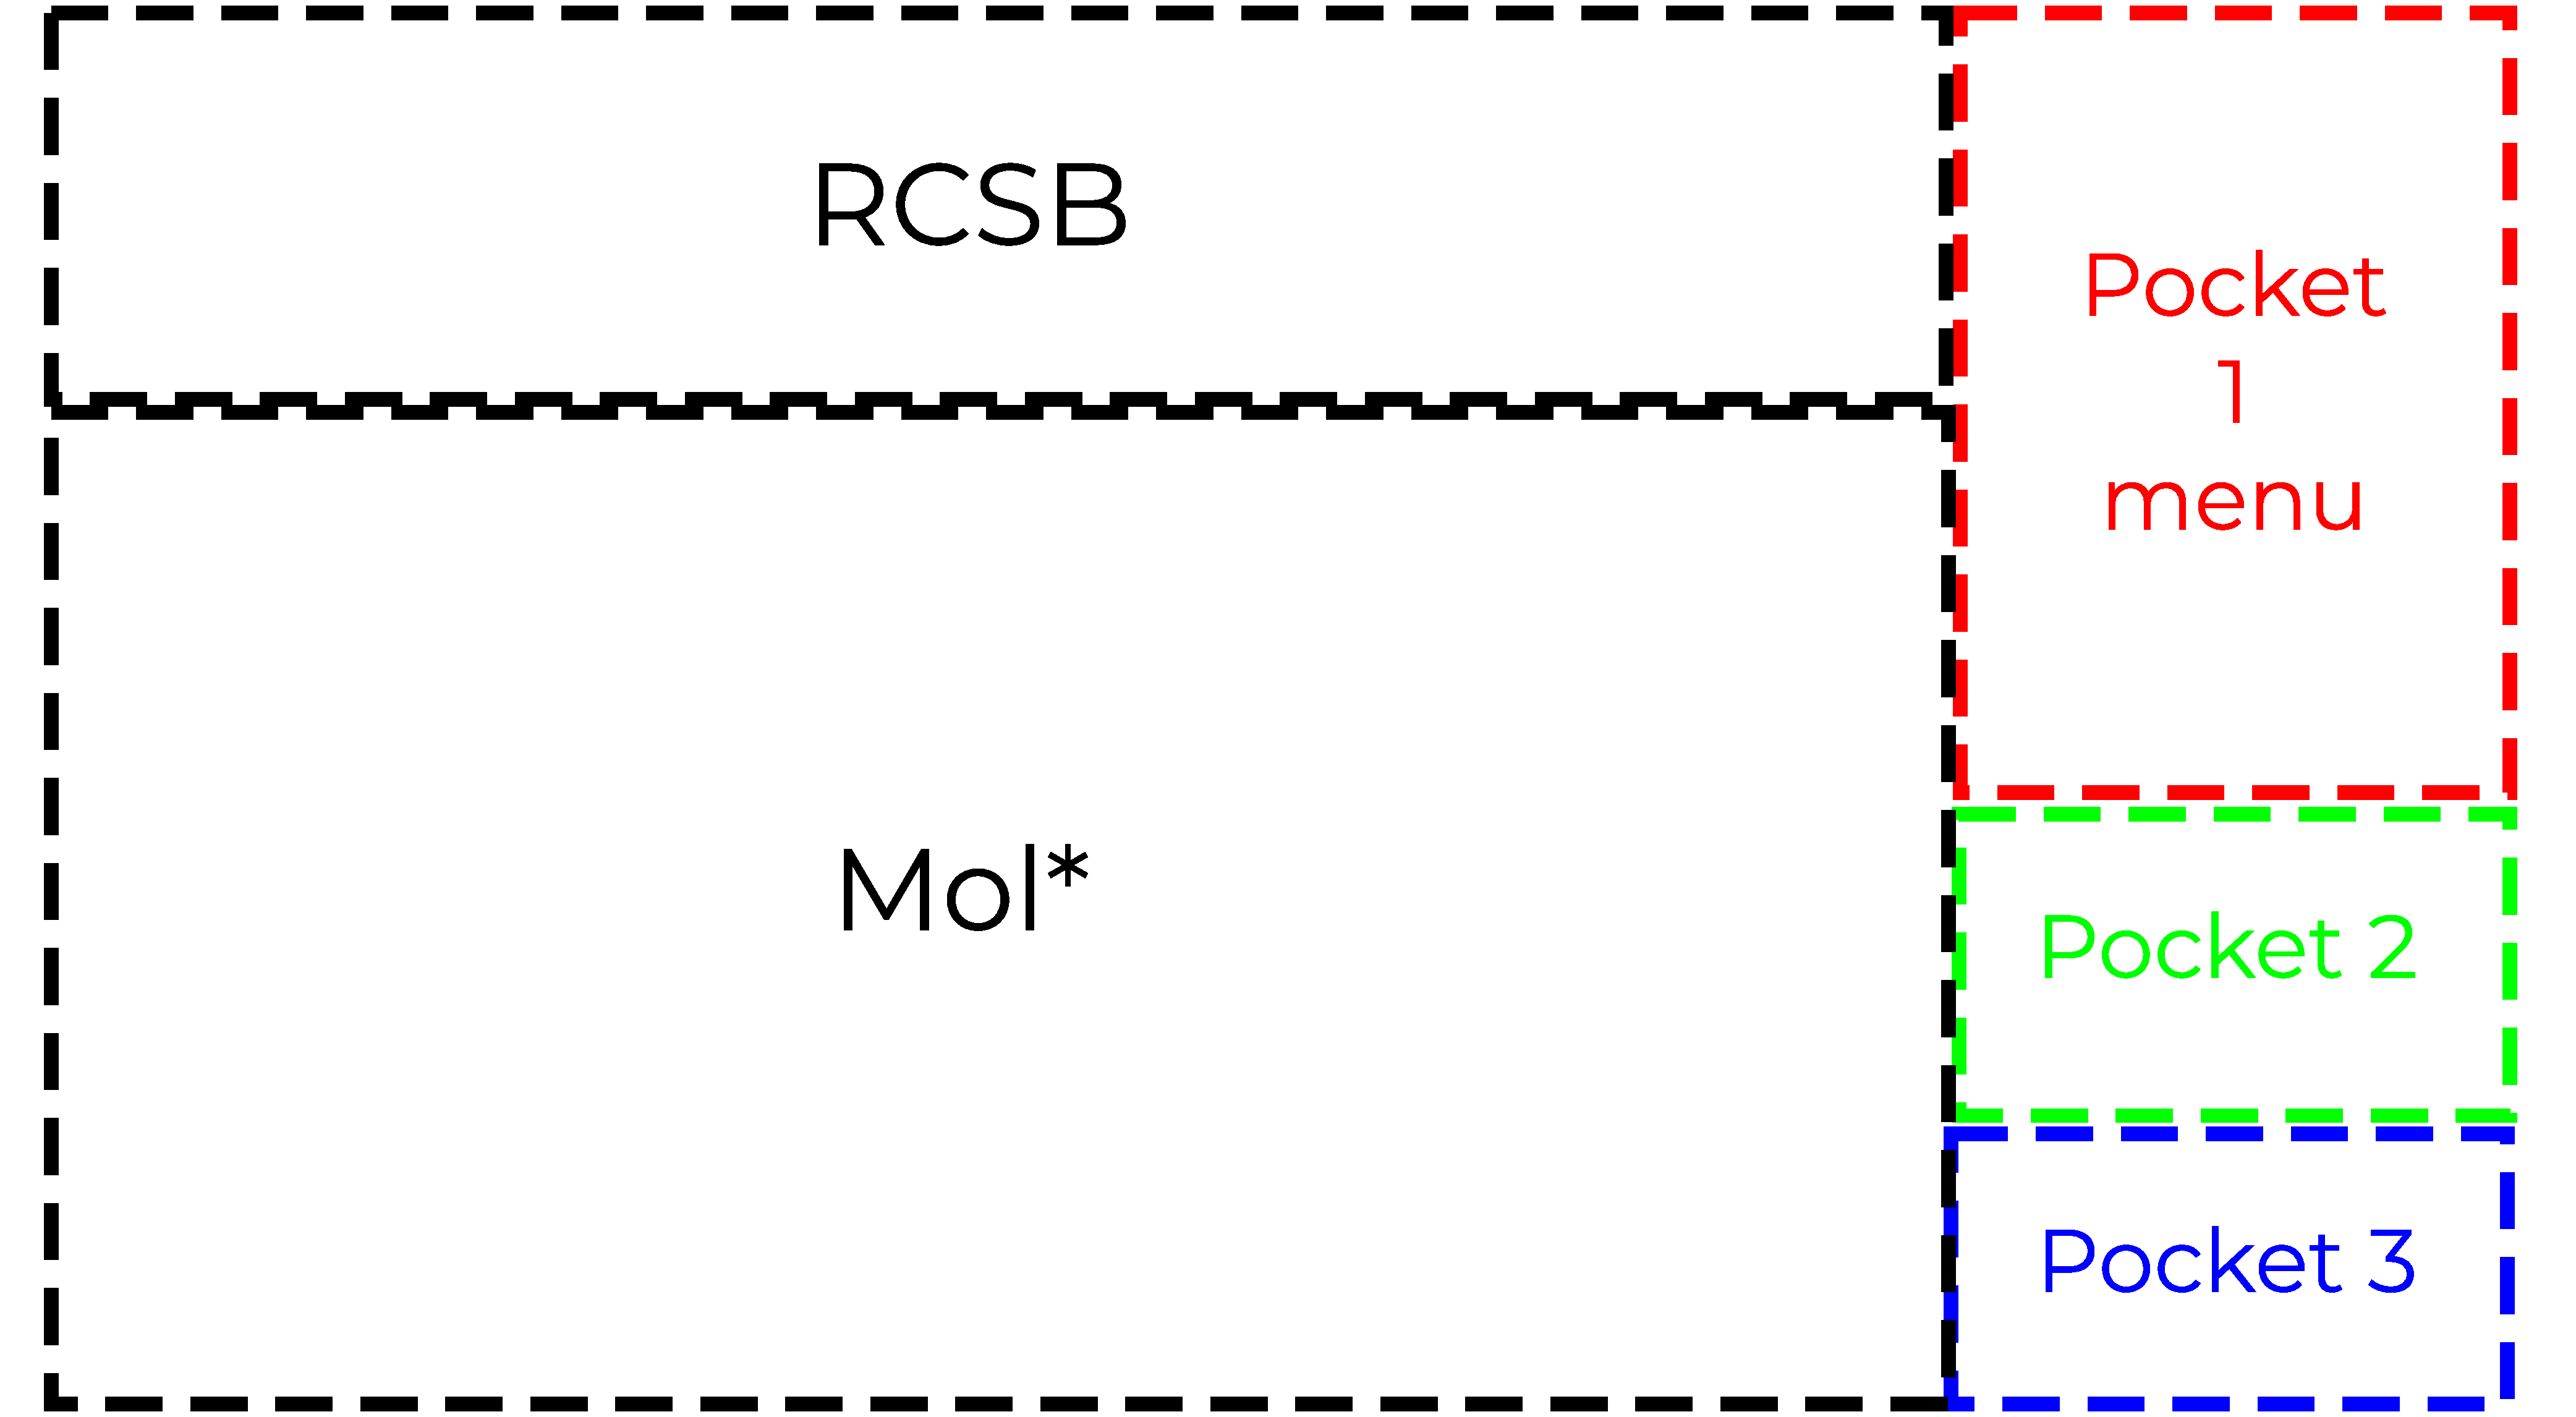
\includegraphics[width=\linewidth]{img/dialog_3-svg.pdf}
	\caption{The third option for displaying detailed pocket information. The tools box is hidden entirely, details of the chosen pocket are displayed in a bigger box on the top. Below this box, other pockets are displayed.}
	\label{fig:dialog-3}
\end{figure}

\begin{figure}[htb]
	\centering
	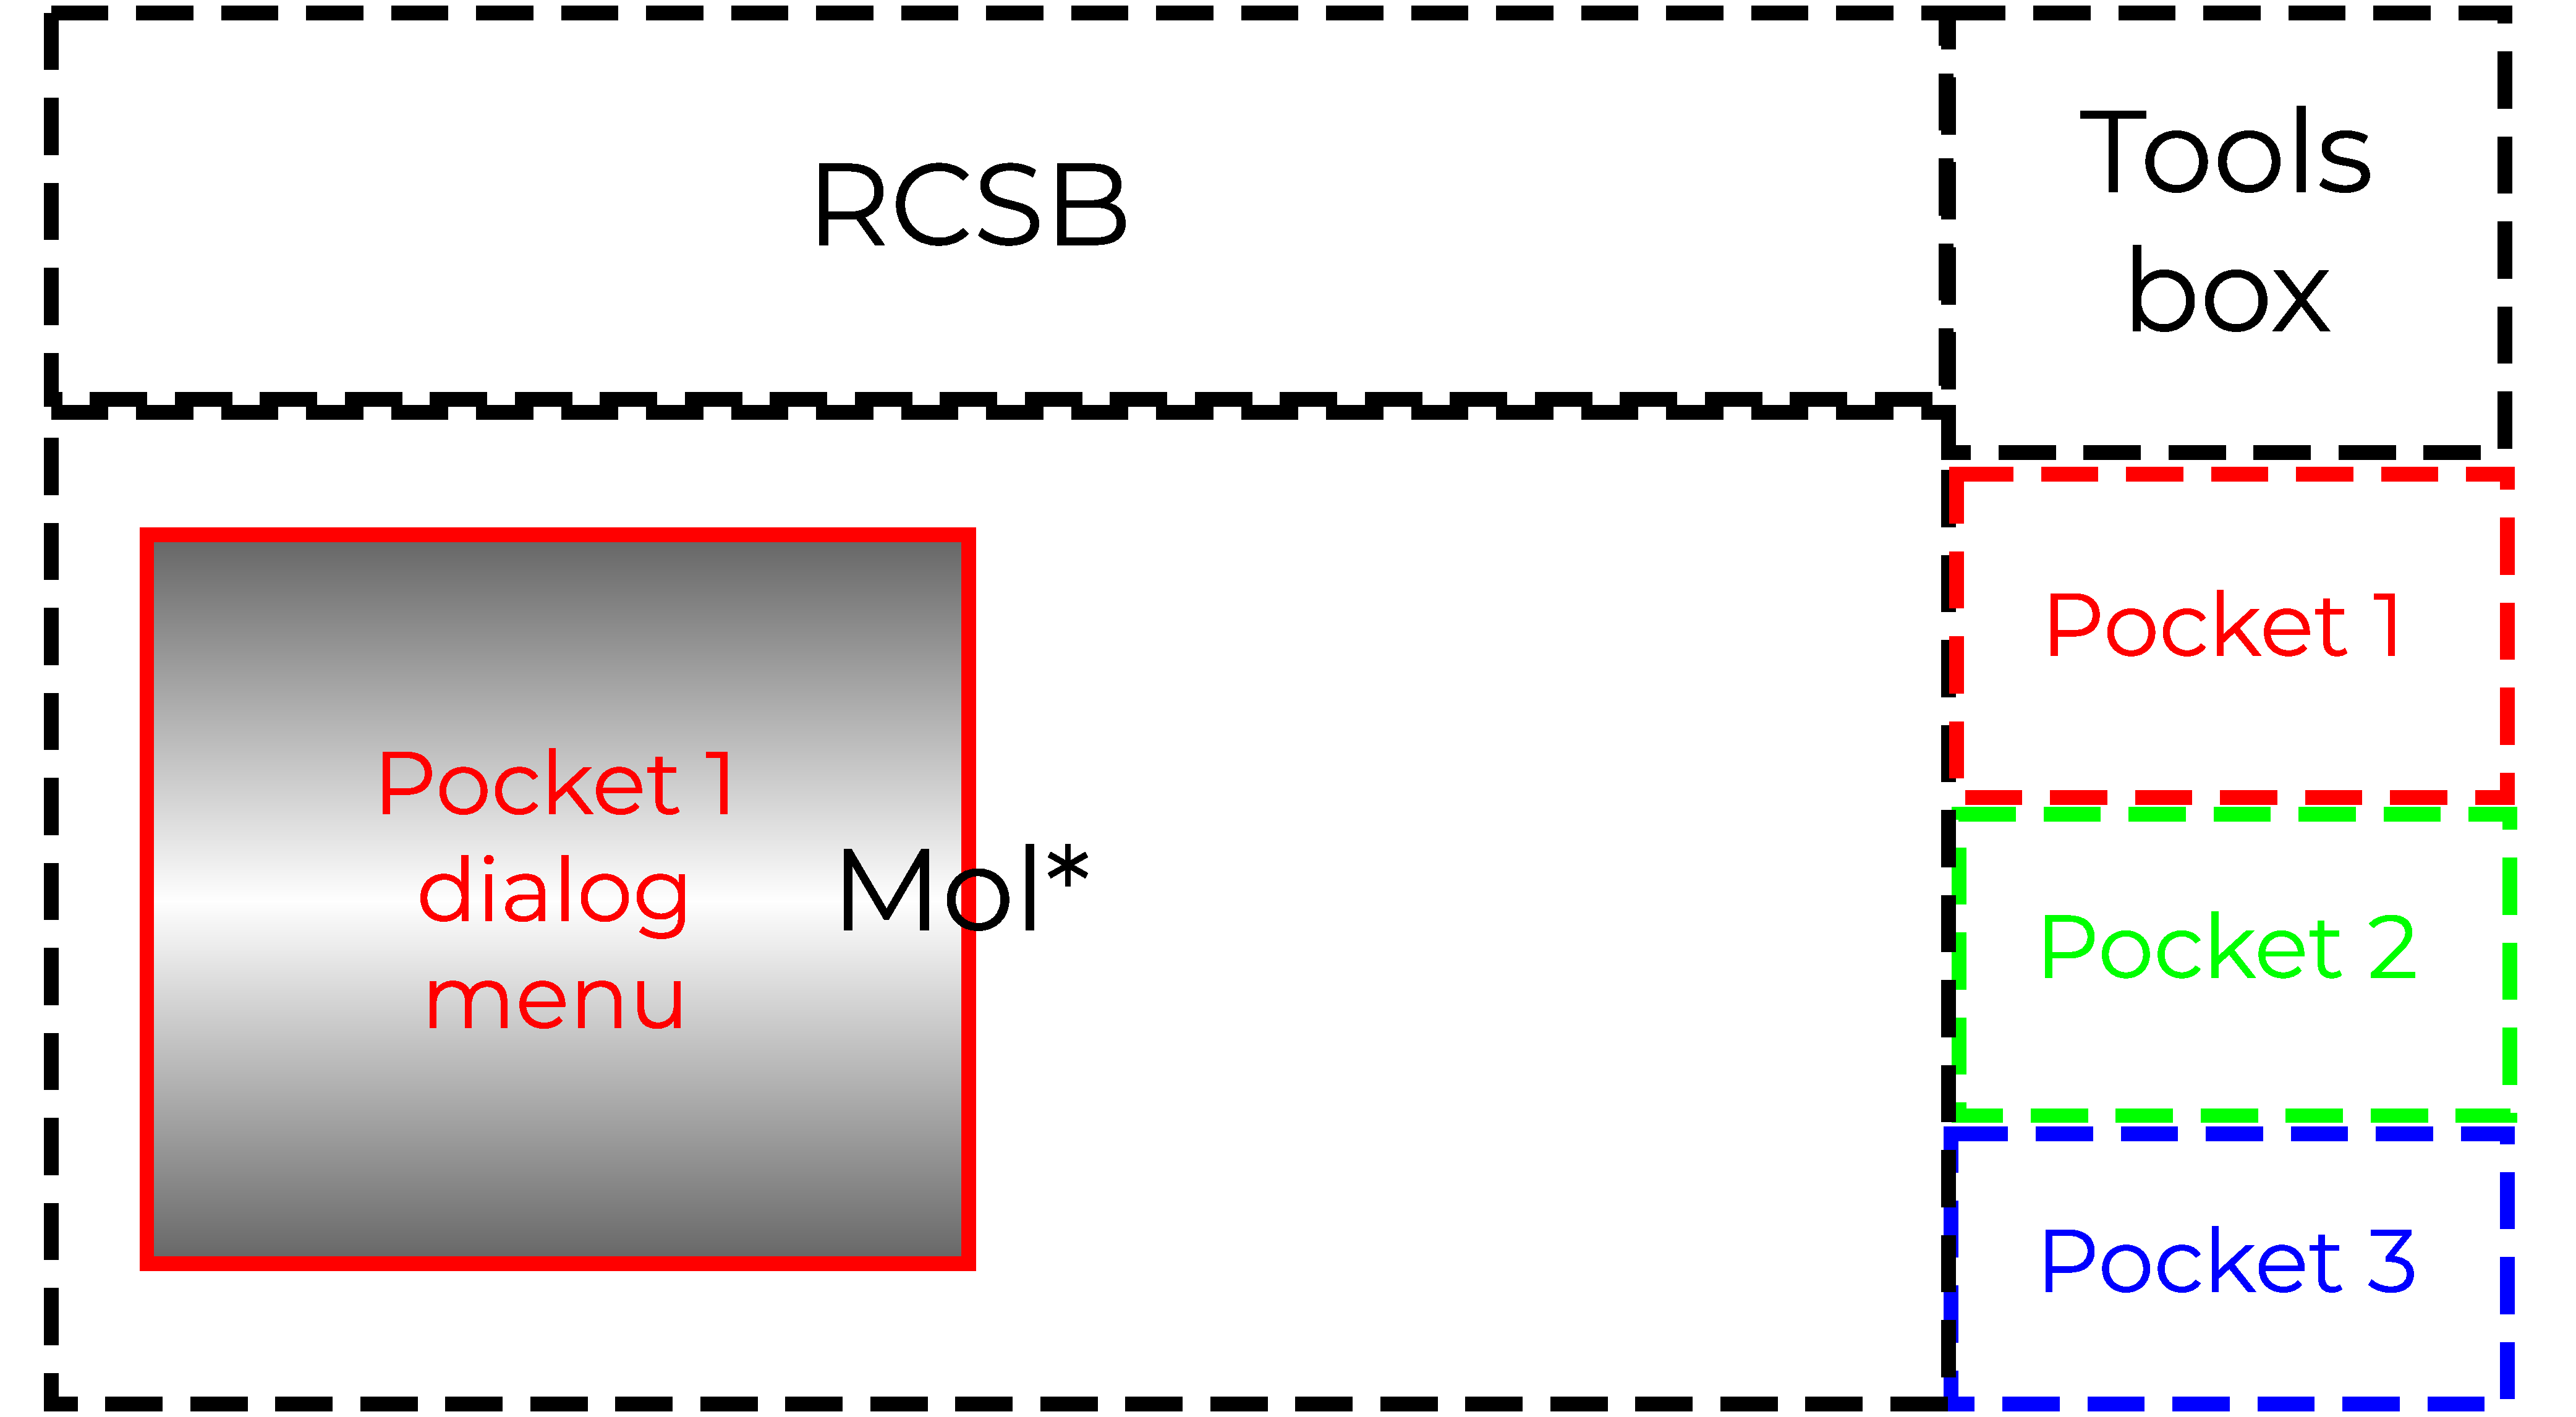
\includegraphics[width=\linewidth]{img/dialog_4-svg.pdf}
	\caption{The fourth (and chosen) option for displaying detailed pocket information. Original design is kept, details of the chosen pocket are shown in a draggable dialog window somewhere on the screen.}
	\label{fig:dialog-4}
\end{figure}
